\chapter{Réduction dimension}

\section{Cadre théorique}
Calculer une matrice de distance entre chacun des points est un classique de la programmation : trouver le plus court chemin, trouver des observations proches pour une distance, clustering en général... Cette opération essentielle est extrêmement coûteuse en temps de calcul et en mémoire. Pour n observations, nous allons devoir calculer n(n - 1) distances, et ça sera encore pire si la distance est en très grande dimension.


Nous avons donc envie d’être capable de réduire la dimension de l’espace dans lequel on travaille, sans pour autant perdre trop d’informations. Nous y verrons plusieurs approches différentes avec des applications différentes, mais qui partage un but commun : réduire la complexité des données sur lesquelles nous travaillons. Naturellement, nous allons perdre de l’information, et nous verrons comment les différentes méthodes traitent cette minimisation de perte d’informations.


Dans le cadre supervisé nous considérions un dataset composé d’un vecteur et la réponse attendue, mais dans le cadre non supervisé nous n’avons que des observations et aucune réponse. 

\newpage


\section{Johnson-Lindenstrauss}
\subsection{Expliquer puis démontrer le lemme}
La première méthode que nous voyons est à la frontière entre les mathématiques et l’informatique théorique. On comprend dans l’annexe D que plus nous sommes en grande dimension, moins la distance a de sens. Ainsi, nous aimerions tout de même conserver les observations proches dans l’espace de départ dans l’espace d’arrivée. Plus formellement, nous cherchons une fonction f : Rd ! Rk avec k << d telle que pour " > 0 et 8(u, v) 2 D2, nous ayons la propriété :
\\
\begin{equation*} (1-\varepsilon)\|u-v\|_2^2 \leqslant \|f(u)-f(v)\|_2^2 \leqslant (1+\varepsilon) \|u-v\|_2^2 \end{equation*}
\\
Cela ressemble à la définition d’une fonction lipschzienne mais sans coefficient unique de lipschitz. Cela ressemble en réalité plus à une distortion d’ordre au plus 1 + ". Cette similitude est expliqué par le titre de l’article Extension of Lipschitz mapping into a Hilbert space publié en 1984 par William Johnson et Joram Lindenstrauss. Être capable de prouver qu’une telle fonction existe, et dire comment nous pouvons la construire est cruciale. De plus, nous sentons que nous allons avoir une dépendance entre la dimension de l’espace d’arrivée k et la distortion maximale que l’on s’autorise $\varepsilon$. Ce papier répond à toutes ces questions via le lemme suivant.
\\
\\
%\lemme{Soit $\varepsilon>0$ et $\mathcal{D} \in \mathbb{R}^{n\times d}$ un dataset avec $d$ colonnes et $n$ lignes/observations. Si $k > \frac{24}{3\varepsilon^2 - 2\varepsilon^3}\ln{n}$, alors il existe une fonction $f: \mathbb{R}^d \rightarrow \mathbb{R}^k$ telle que :
\\
\begin{equation*} 
(1-\varepsilon)\|u-v\|_2^2 \leqslant \|f(u)-f(v)\|_2^2 \leqslant (1+\varepsilon) \|u-v\|_2^2 
\end{equation*}
pour tout $(u, v) \in \mathcal{D}^2$.


Commençons par observer que la dimension de l’espace de réduction de dépend pas de la dimension de l’espace de départ ! Une manière de saisir pourquoi c’est bien que le cas est que si n > d alors nous pouvons plutôt considérer l’espace engendré par les n observations plutôt que d. Nous sommes bien dans un des pires scénarios, mais la borne sur k tient toujours. Remarquons de plus que le résultat est vrai, peut importe la nature de D, ce qui rend le lemme encore plus général.


Avec le tableau ci-dessous nous pouvons voir les dimensions minimale de l’espace de réduction en fonction de $n$ et $\varepsilon$.


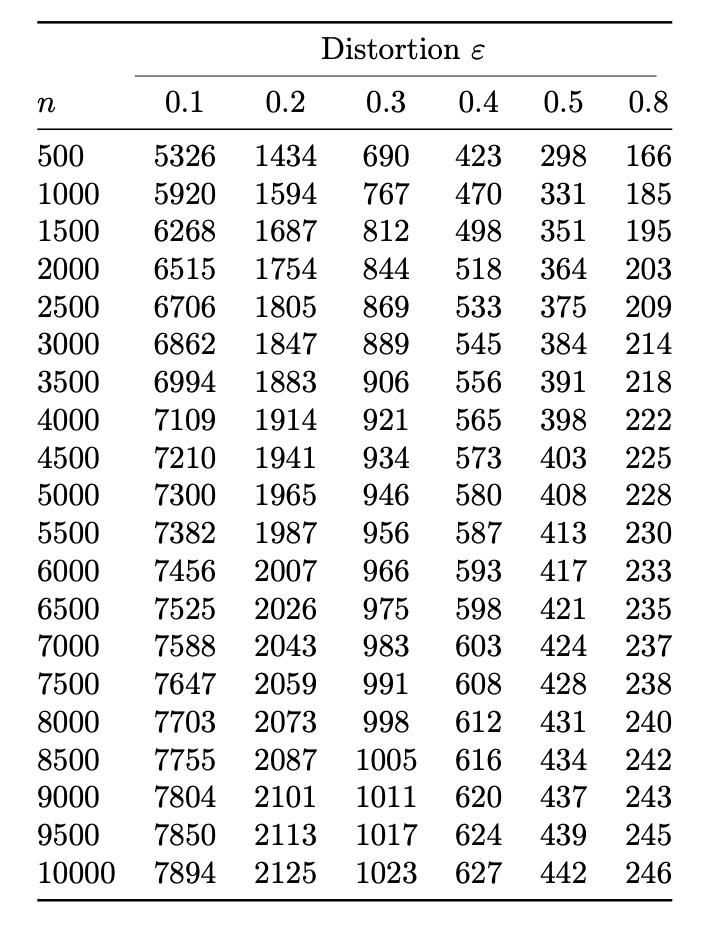
\includegraphics[width=200pt]{./img/reduction_dim/lemme_jl/table}


Nous sentons la progression logarithmique en nombre d’observations : seulement 48\% d’augmentation de l’espace de réduction pour $\varepsilon$ entre n = 500 et n = 10000 qui représente une augmentation de 1900\% en n.
On observe également le comportement prévisible de l’évolution en $\varepsilon$ qui n’est pas linéaire. Etudions un peu plus la valeur de k :


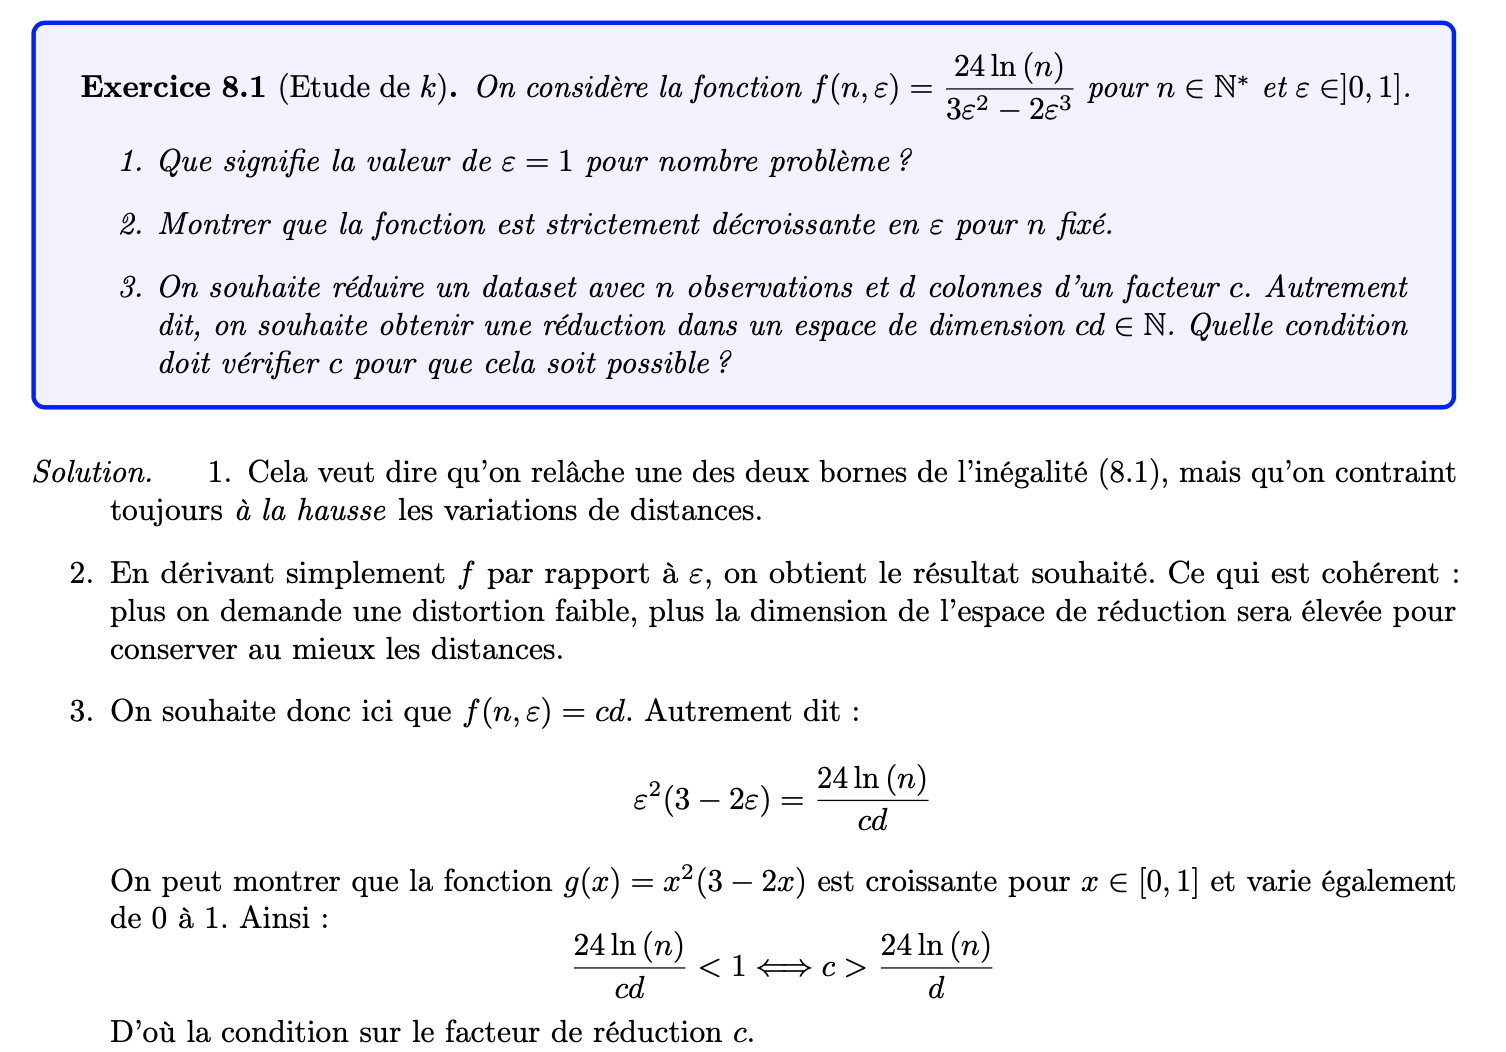
\includegraphics[width=\linewidth]{./img/reduction_dim/lemme_jl/exercice_jl}


Remarquons que le lemme n’est pas toujours avantageux : pour n = 500 et $\varepsilon$ = 0.1, on ne peut pas projeter le dataset dans un espace de dimension plus petit. Pour le faire il faut accepter une distortion d’au moins 0.4.
\\
Avec uniquement le lemme, nous savons qu’une telle fonction existe et quel est la réduction de dimension que l’on peut obtenir. Mais nous ne savons pas comment construire une telle fonction. On obtient la réponse en démontrant le lemme puisque nous pouvons le faire via une démonstration par construction. 
\\
Nous ne le ferons pas ici, mais nous pouvons noter qu’il existe de très nombreuses manière de construire une telle fonction et qu’il s’agit d’un domaine de recherche en informatique.


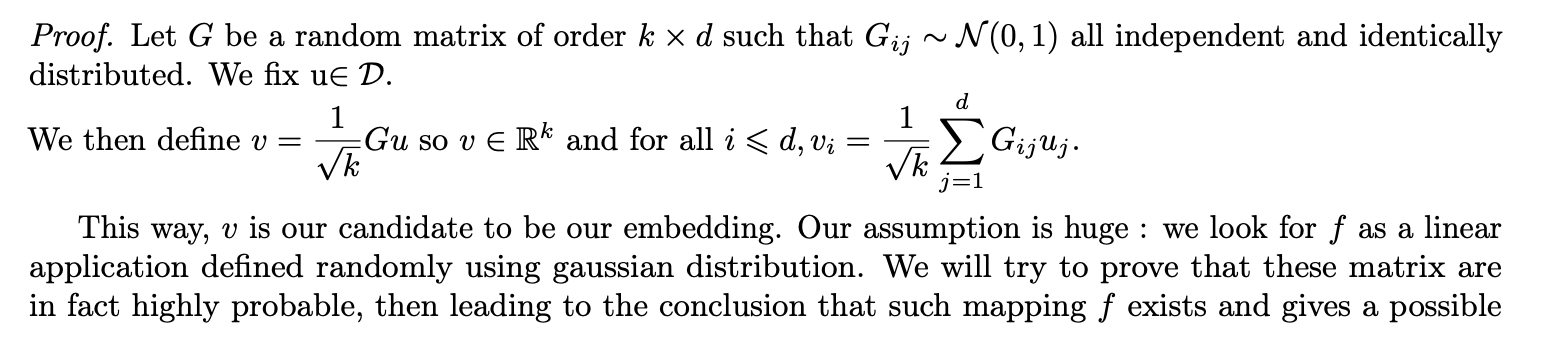
\includegraphics[width=\linewidth]{./img/reduction_dim/lemme_jl/preuve_1}
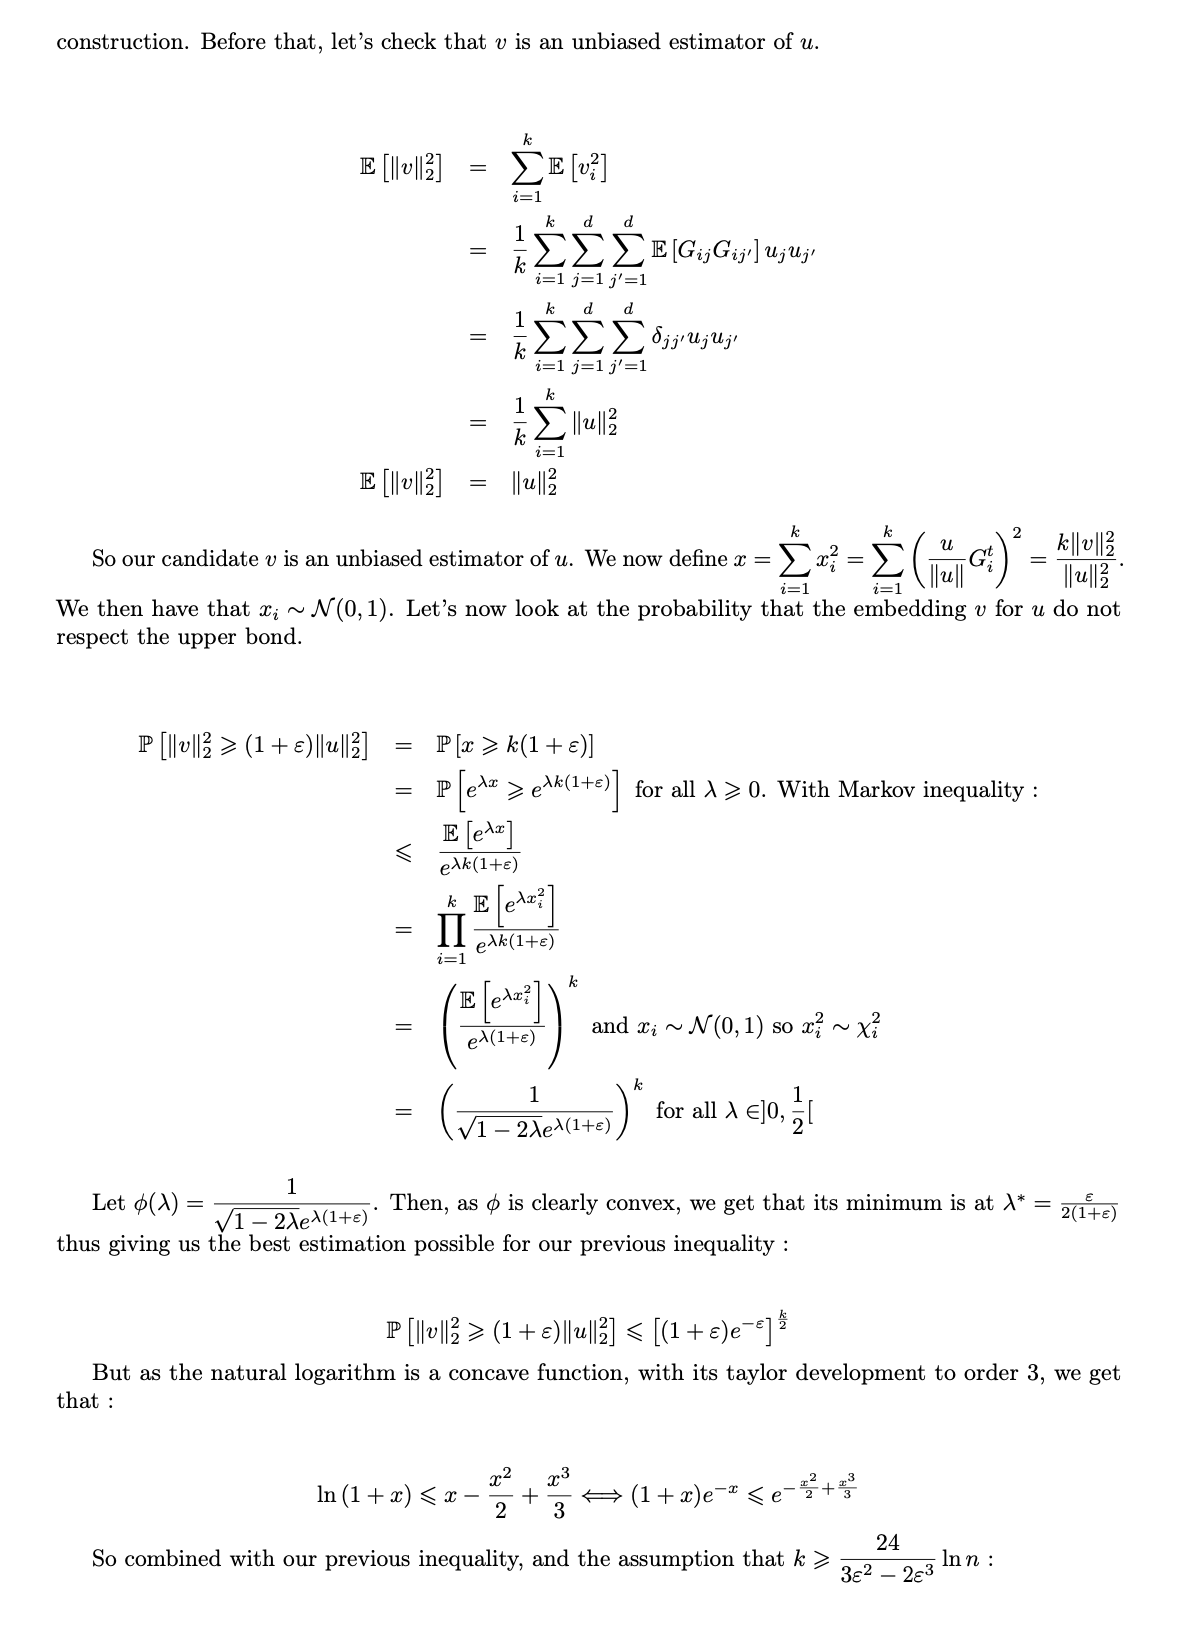
\includegraphics[width=\linewidth]{./img/reduction_dim/lemme_jl/preuve_2}
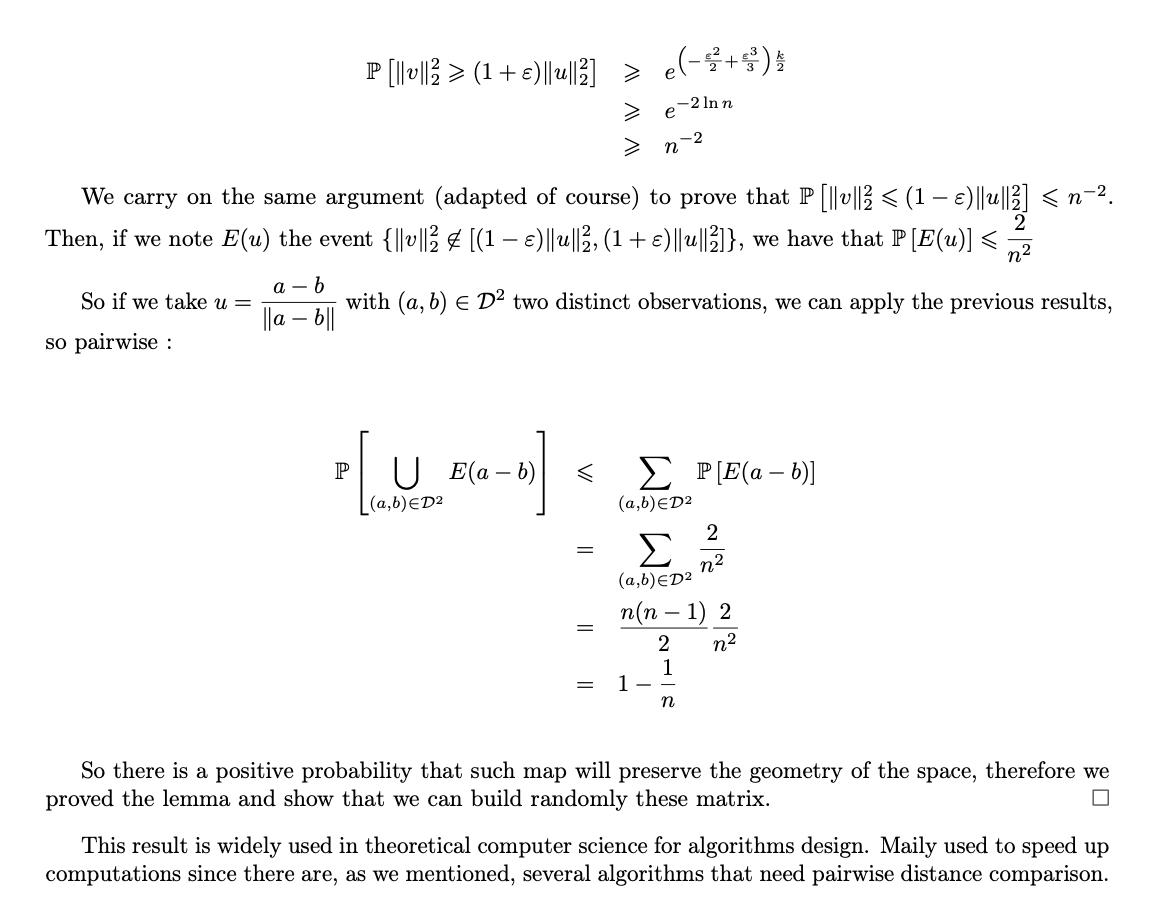
\includegraphics[width=\linewidth]{./img/reduction_dim/lemme_jl/preuve_3}
\\
\\
Ce qui est important de noter, c’est que chacune des preuves de ce résultat construit la fonction f solution en faisant apparaître des projections aléatoire. Autrement dit, en projetant aléatoirement (mais en choisissant bien son aléatoire) dans un espace de dimension k nous pouvons réduire très facilement la dimension de l’espace de départ.
\\
Ce résultat est très largement utilisé en informatique théorique pour le design d’algorithme qui exploitent de très large base de données. Ce résultat est essentiellement utilisé pour accélérer les temps de traitement des algorithmes qui ont besoin de calculer des distances entre chacune des observations de la base.
\\
Les constructions, pour la preuve, peuvent être optimisées pour accélérer encore plus les calculs. Dans la preuve que nous avons faites, nous avons utilisé une matrice dense de variables aléatoire gaussienne : c’est coûteux à la fois en taille et en temps de génération. Dans Database-friendly random projections : Johnson-Lindenstrauss with binary coins, Dimitri Achlioptas montre en 2003 que l’on peut avoir le même résultat avec une matrice avec $\frac{2}{3}$ des entrées vide et uniquement remplie avec des valeurs +1 et -1. C’est bien moins volumineux pour le stockage et rapide à générer.
\\
La meilleure borne a été proposé par Kane Daniel et Nelson Jelani en 2014 dans Sparser Johnson- Lindenstrauss Transforms où la borne ne peut pas être améliorée. En pratique, il y a encore beaucoup de travail sur ce lemme puisque nous n’avons considéré que la distance euclidienne. Si nous travaillons avec la distance manhattan, alors ce résultat ne tient plus. De manière générale pour les normes Lp le résultat n’est pas vrai. Même si la norme euclidienne est de loin la plus utilisée, la norme L1 a plus de sens en grande dimension comme nous l’avons vu avec la régression LASSO.
\\
\\
Pour notre problématique de Machine Learning, ce lemme est utile puisqu’il peut permettre de mieux stocker par exemple des données vidéos, mais il y a plusieurs inconvénients :
\begin{itemize}
    \item La dimension de l’espace de réduction reste élevée pour une visualisation en très petite dimension.
    \item A ce jour, les projections sont faite aléatoirement, donc sans procédure intelligente.
    \item Il n’y a pas de maîtrise du datascientist autre que par le paramètre $\frac{2}{3}$ des projections.
\end{itemize} 
Ces trois points sont pourtant quelque chose que nous souhaiterions obtenir. Il nous faut donc développer d’autre manière de réduire la dimension.


\newpage


        \subsection{Visualiser (un peu)}
        Visualisation


        \newpage













    \section{PCA}
        \subsection{Expliquer la théorie/différence avec Johnson-Lindenstrauss}
            Dans l’analyse par composantes principales il est question d’identifier les directions qui expliquent le mieux les variations des données. Si l’on suppose que les données, par exemple, se distribue uniformément au sein d’une ellipse, nous identifions clairement les axes comme dans la figure ci-dessous :
            \\
            \\
            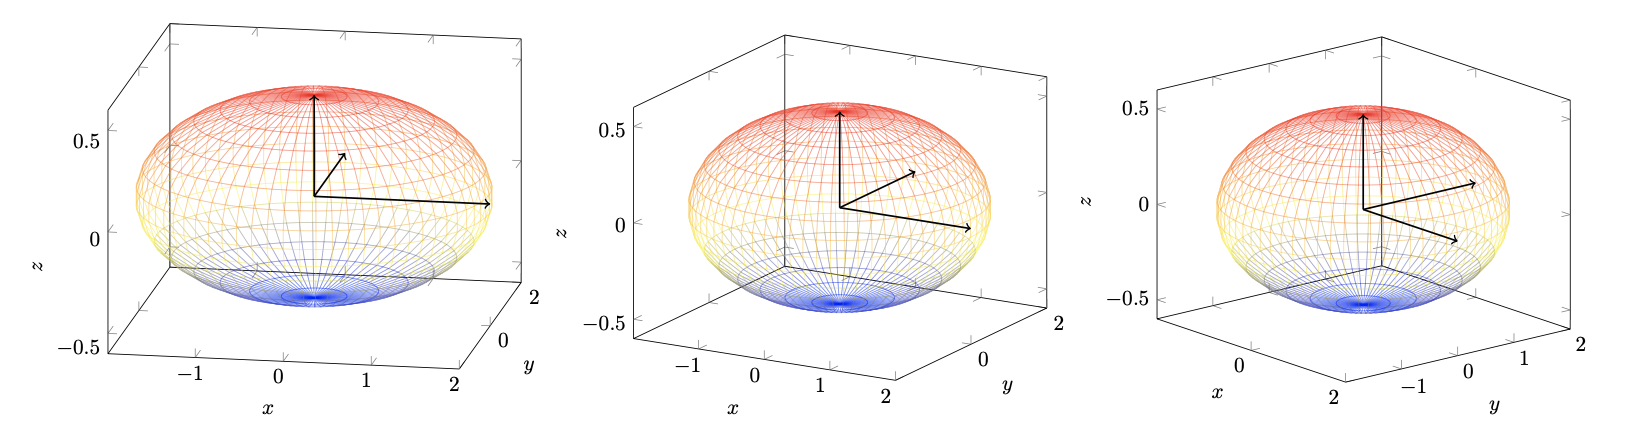
\includegraphics[width=\linewidth]{./img/reduction_dim/pca/elipse}
            \\
            \\
            L’objectif est donc de définir comment trouver ces axes qui nous semblent évident en petite dimension parce que nous sommes capable de les voir, mais cette fois en grande dimension. Si nous sommes capable de les trouver, nous seront en capacité de définir un nouveau repère pour exprimer les informations que nous avons. Ainsi, fort de cette base, nous pourrons sélectionner un échantillon de ses axes pour produire des graphiques compréhensible par l’humain.
            \\
            \\
            Voici les questions auxquelles nous devons répondre :
            \begin{enumerate}
                \item Comment trouver les directions qui décrivent le mieux les variations ?
                \item Comment s’assurer que les directions formeront bien une nouvelles bases ? 
                \item Comment prioriser les directions ?
            \end{enumerate}
            On remarque que les questions ne sont pas toutes bien posées, et nous devons nous laisser guider pour les affiner. Les réponses se trouve dans des notions fondamentales d’algèbre.



                \subsubsection*{Diagonalisation d’une matrice}
                    Soit la matrice $A$ définit comme :
                    \\
                    \begin{eqnarray*}
                         A = \frac{1}{2} \left(\begin{array}{cc}3 & 1 \\ 1 & 3\\\end{array}\right)
                    \end{eqnarray*}
                    \\
                    On sait que si l’on prend un vecteur $u \in \mathbb{R}^2$, on peut multiplier la matrice $A$ par $u$ : on dit en algèbre que $A$ agit sur $u$. Visualisons ce que cela veut dire géométriquement.
                    \\
                    \\
                    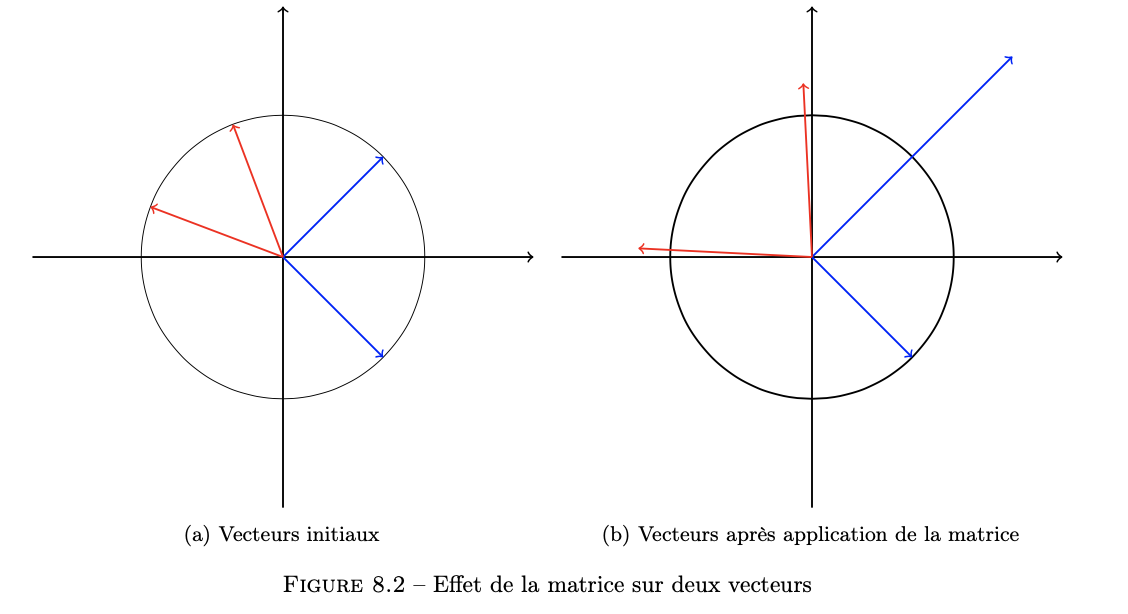
\includegraphics[width=\linewidth]{./img/reduction_dim/pca/vect_prp}
                    \\
                    \\
                    On remarque que les deux vecteurs rouges on changé de direction et de taille, là où les vecteurs bleus ont conservés leurs direction (mais pas nécessairement leurs taille). C’est étonnant d’avoir une invariance de direction pour seulement ces deux directions là (on peut le vérifier par le calcul). Ces deux vecteurs bleus semblent être des vecteurs particuliers pour la matrice A. Généralisons.
                    \\
                    \\
                    On considère une matrice carré A de taille $n$ dans l’ensemble de la section.
                    \\
                    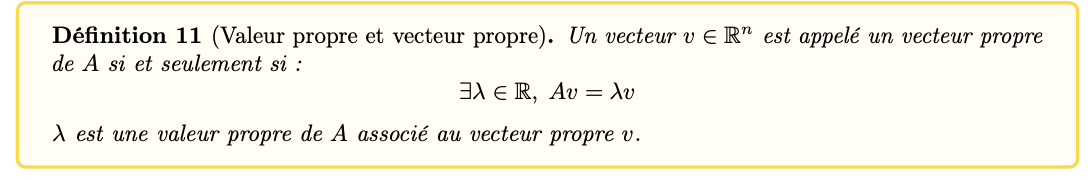
\includegraphics[width=\linewidth]{./img/reduction_dim/pca/def_val_prp}
                    \\
                    Dans notre exemple, le vecteur (1, 1) est un vecteur propre de A ! Et sa valeur propre $\lambda$ est 2. Pour le vecteur (1, -1) sa valeur propre est 1, d’où le non changement d’échelles. Remarquons que si $v$ ne doit pas être nul pour être un vecteur propre, $\lambda = 0$ est autorisé.
                    \\
                    \\
                    Non unicité d’un vecteur propre : soit $\lambda$ une valeur propre de A associé à un vecteur propre $v$. On sait qu’il existe une infinité de vecteur propre lié à la valeur propre $\lambda$.
                    \\
                    Par définition, on a que $Av = \lambda v$, donc si on multiplie par une constante $c \in \mathbb{R}^*$, l’équation devient $cAv = c \lambda v \iff A(cv) = \lambda (cv)$ d’où $cv$ est un vecteur propre de $A$.
                    \\
                    Suite à cette remarque, on comprend que nous n’obtiendrons l’unicité pour un vecteur propre qu’en imposant des règles. Les plus classiques demandes à ce que le vecteur soit de norme 1, mais ça ne garanti par l’unicité encore.
                    \\
                    \\
                    \textbf{Comment trouver les valeurs propres d’une matrice ?}
                    \\
                    (Caractérisation des valeurs propres). $\lambda \in \mathbb{R}$ est une valeur propre de $A$ si et seulement si :
                        $det(\lambda In - A) = 0$
                    \\
                    \\
                    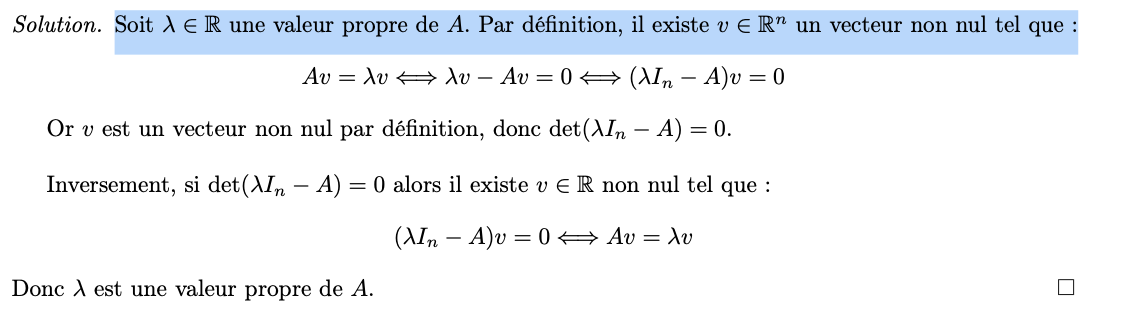
\includegraphics[width=\linewidth]{./img/reduction_dim/pca/prv_val_prp}
                    \\
                    \\
                    Donc $\lambda$ est une valeur propre de $A$.
                    \\
                    \\
                    On appelle l’équation définie dans le théorème (Caractérisation des valeurs propres) l’équation caractéristique de $A$.
                    \\
                    Le polynôme en $\lambda$ issue de cette équation est de degré au plus $n$, et donc nous sommes certains d’avoir $n$ racines complexes, potentiellement complexes et potentiellement répétées. Ici, nous avons donc bien nos deux vecteurs bleus qui sont les seuls vecteurs propres de la matrice $A$ de l’exemple.
                    \\
                    \\
                    Maintenant que nous sommes capables de trouver l’ensemble des valeurs propres d’une matrice, en résolvant l’équation $Av = \lambda v$ en $v$ et en sélectionnant les vecteurs propres de norme 1, nous sommes également capable de calculer l’ensemble des vecteurs propres.
                    Un résultat (que nous ne démontrerons pas) nous informe que cette ensemble de vecteur propre forme une base, autrement dit, les vecteurs sont de norme 1 et orthogonal entre eux. Ainsi, on définit :
                    \\
                    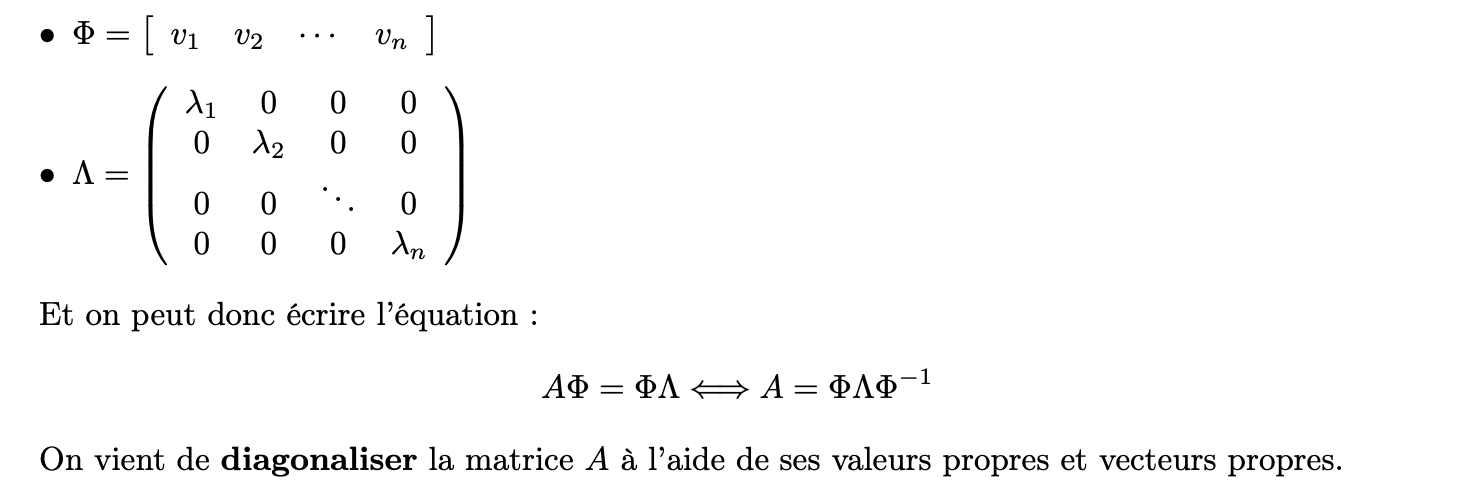
\includegraphics[width=\linewidth]{./img/reduction_dim/pca/mat_diag}
                    \\
                    \\
                    \textbf{(Puissance d’une matrice) Soit A une matrice diagonalisable de taille d. Calculer $A^n \in \mathbb{N}$ :}
                    \\
                    Puisque $A$ est diagonalisable, il existe $\Phi$ et $\Lambda$ défini comme précédemment telle que $A = \Phi \Lambda \Phi^{-1}$. Par récurrence rapide, on peut montrer que :
                    \\
                    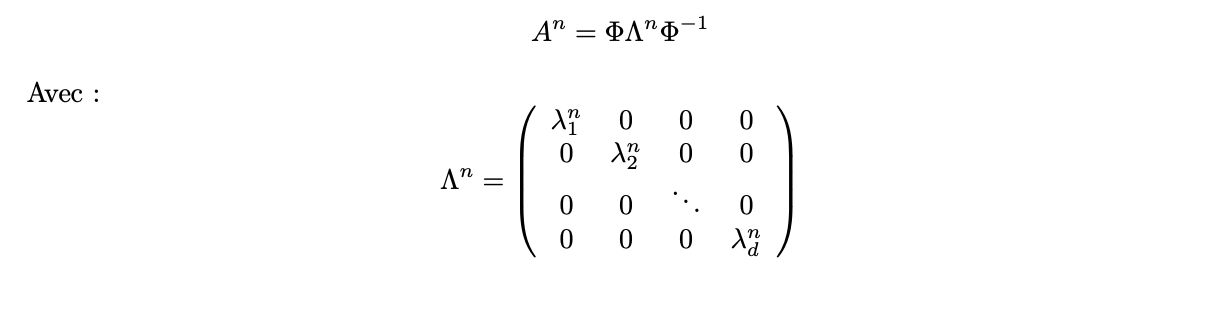
\includegraphics[width=\linewidth]{./img/reduction_dim/pca/mat_puissance}
                    \\
                    C’est un résultat qui permet d’accélérer très nettement les calculs de puissance de matrice puisque nous n’avons besoin de calculer que deux multiplications de matrice, au lieu de $n$. Mais on pourrait se dire que calculer l’inverse de la matrice $\Phi$ coûte. En pratique, comme nous avons une base, $\Phi^{-1} = \Phi^t$.
                    \\
                    \\
                    Voyons sur un exemple comment l’analyse par composante principale nous permet de mieux visualiser une matrice :
                    \\
                    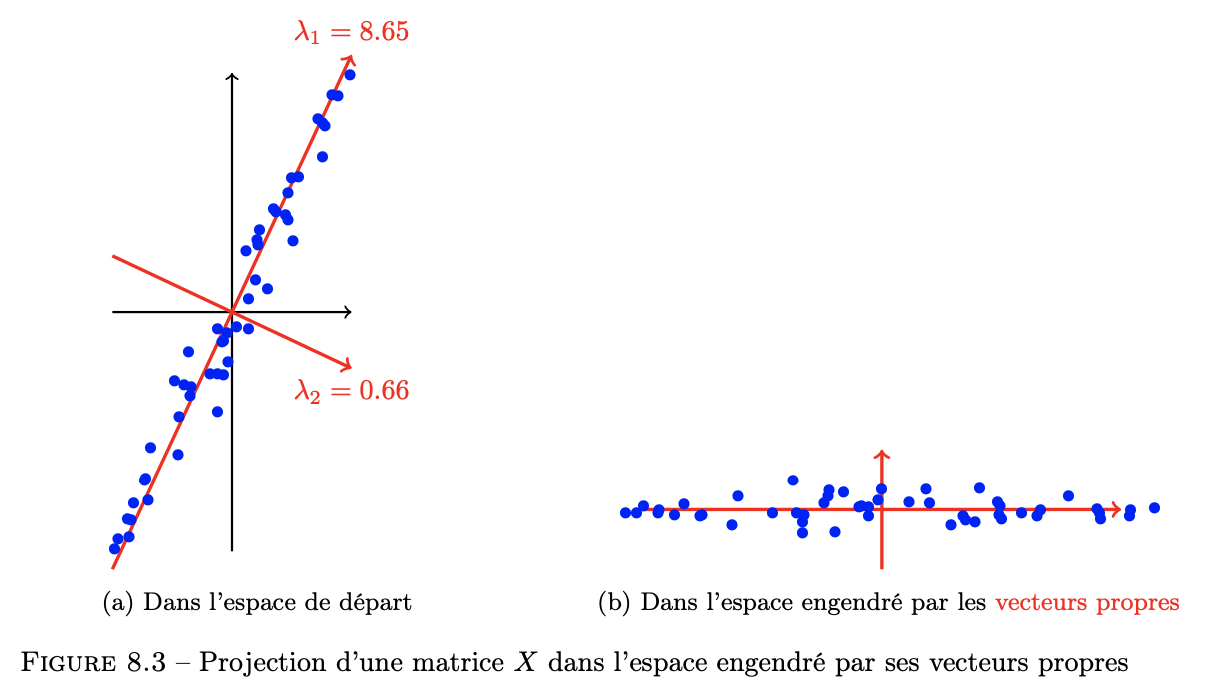
\includegraphics[width=\linewidth]{./img/reduction_dim/pca/graph_mat}
                    \\
                    Dans la figure ci-dessus, on présente la projection de l’espace de départ (engendré par $X$) et l’espace défini par les vecteurs propres de $X$. C’est exactement ce que l’on voulait : le grand axe de variation a été comprit, et les deux vecteurs propres forment une base orthonormée pour projeter $X$. Ainsi, on peut se suffire de la composante liée à $\lambda_1$ pour bien approcher les variations de la matrice : on a bien réduit la dimension.



                \subsubsection*{Application à la réduction de dimension}
                    C’est cette dernière remarque qui motive notre utilisation de ces résultats d’algèbre. Nous pouvons projeter $X$ dans un sous-ensemble de ses vecteurs propres et conserver a priori le plus de variations expliquées. Se posent alors deux questions :

                    \begin{enumerate}
                        \item Est-t-on certain que l’on pourra toujours diagonaliser X ?
                        \item Comment prioriser les composantes à conserver ?
                    \end{enumerate}

                    La première question est répondu par la négative : il n’y a aucune garantie mathématiques qu’une matrice quelconques puissent être diagonalisable. $X$ n’est même pas une matrice carré en règle général ! Puisqu’on cherche à identifier les axes où la variance est la plus forte, décomposons la matrice de variance-covariance de $X$ ! On la note $\Sigma $et dans notre cas, elle se définit comme :
                    \\
                    \\
                    \begin{eqnarray*}
                        \Sigma = \frac{XX^t}{n - 1}
                    \end{eqnarray*}
                    \\
                    \\
                    Chaque coefficient $(\sigma_{ij})_{1 \leqslant i, j \leqslant d}$ de $\Sigma$ représente la covariance entre l’information $i$ et l’information $j$. Ainsi, quand $i = j$, cela revient à avoir la variance de l’information $i$, d’où le nom de matrice de variance-covariance. Cela fait déjà plus de sens philosophiquement, et on a cette fois la garantie de toujours pouvoir la diagonaliser puisque $\Sigma$ est une matrice symétrique semi-définie positive.
                    \\
                    \\
                    Il reste à savoir comment prioriser les composantes à conserver. On remarque dans la figure (8.3) que les valeurs propres associées à chacun des axes sont très différentes et on dirait que la valeur est corrélées à l’importance de la direction.
                    Voyons avec un exercice comment nous pouvons tirer partie de cette information.
                    \\
                    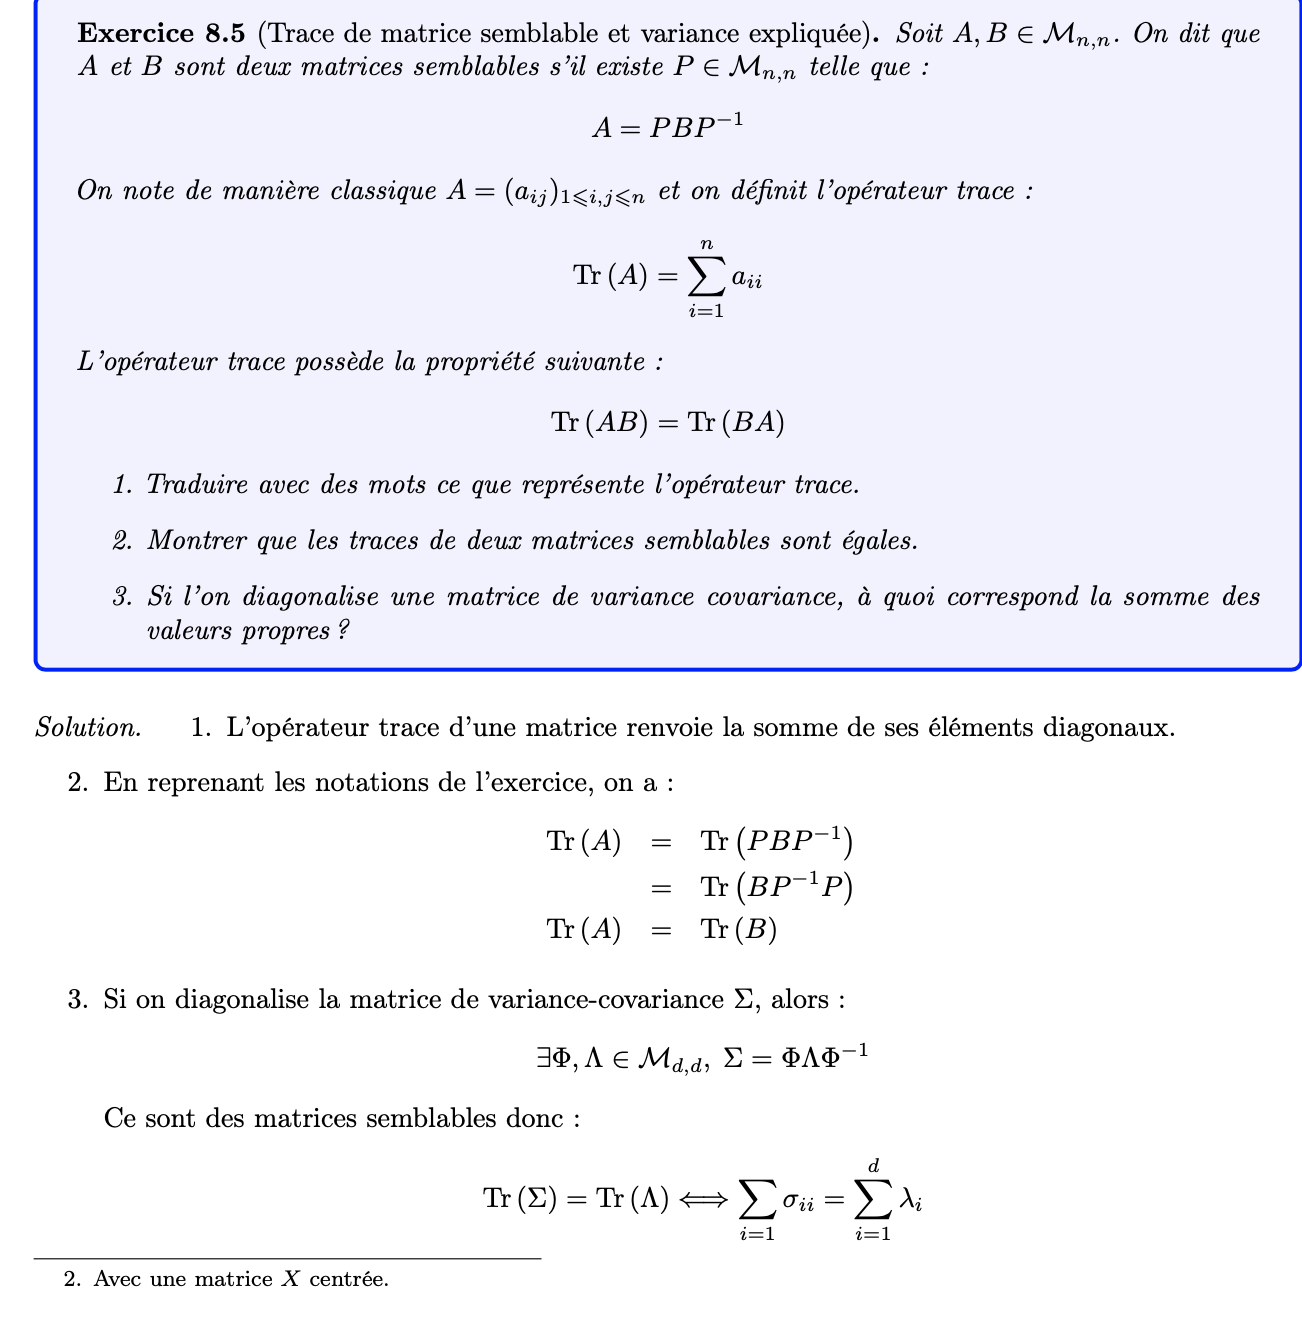
\includegraphics[width=\linewidth]{./img/reduction_dim/pca/mat_trace}
                    \\
                    Autrement dit, la somme des variances de chacune des informations contenues dans la matrice $X$ est égale à la somme des valeurs propre de la matrice de variance-covariance.
                    \\
                    \\
                    Avec cet exercice on comprend comment nous allons prioriser les axes à conserver : plus une valeur propre est grande, plus sa composante associée est importante. De plus, nous sommes capable de définir la proportion de variance expliquée par chacune des composantes.
                    \\
                    Par exemple, dans la figure (8.3), la première composante explique 93\% de la variance. D’où notre intuition de dire qu’il suffisait de conserver uniquement la première composante pour mieux visualiser les données.
                    \\
                    \\
                    Par rapport au lemme de Johnson-Lindenstrauss, cette fois nous sommes capable d’expliquer chacun des axes créés avec une procédure intelligente. En revanche, nous faisons l’hypothèse que les variations peuvent être expliquées par une combinaison linéaire des informations présentes, ce qui n’est pas forcément le cas.
                    \\
                    \\
                    Finalement, l’analyse par composante principale cherche à résumer la forme de la matrice avec une vision macro via une explication de la variance. Que faire si nous souhaitons réduire la dimension en conservant une vision plus micro cette fois ?


        \newpage





        \subsection{Visualisation}
        Visualisation


        \newpage








    \section{Nouvelle approche : t-SNE}
        \subsection{Cadre théorique}
        T-Distributed Stochastic Neighbor Embedding (t-SNE) a été développé par Laurens van der Maaten et Geoffrey Hinton en 2008. La principale différence avec PCA est que t-SNE est un algorithme de réduction de dimension non linéaire. Ce que cela signifie, c'est que cet algorithme permet de séparer des données qui ne peuvent être séparées par des lignes droites.
        \\
        \\
        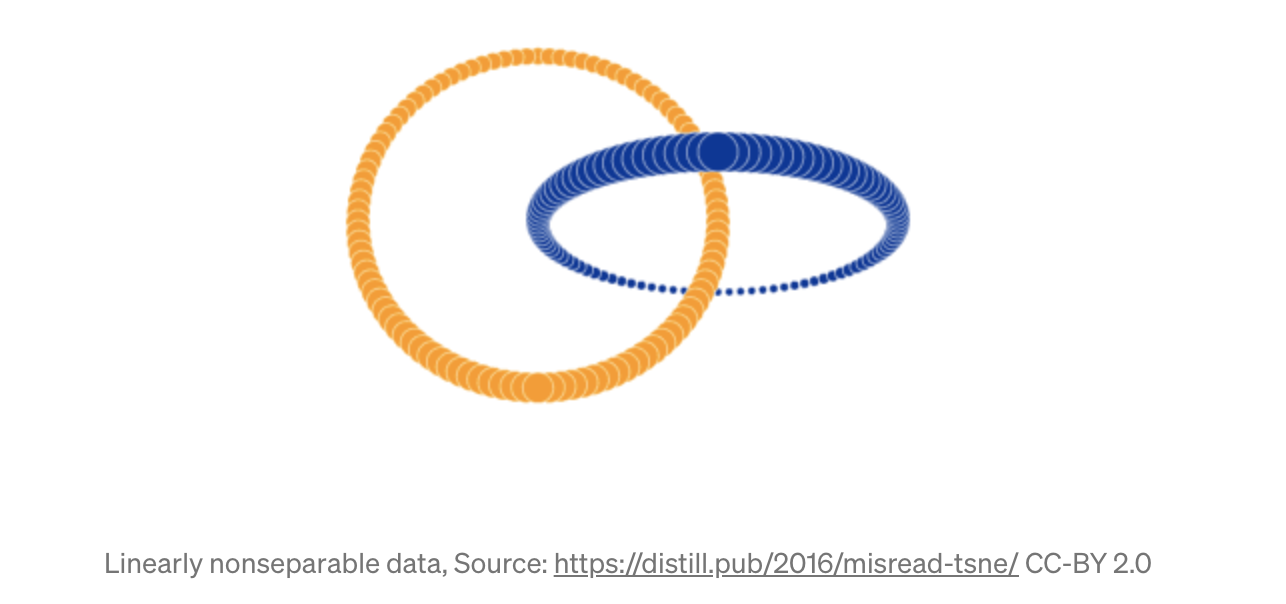
\includegraphics[width=\linewidth]{./img/reduction_dim/t_sne/exemple_data}
        \\
        \\
        Comme le montre cet exemple, il n'est pas possible de séparer ces données de manière linéaire. C'est pour cela que l'utilisation de t-SNE est pertinente dans ce cas précis comparé à PCA.
        \\
        \\
        Ici, la descente de gradient est utilisée pour réduire le graphe en faible dimension dans lequel la distance relative entre les points i et j correspond à celle de l'espace original de haute dimension ; sous le contrôle d'un paramètre de perplexité qui détermine l'écart-type des distributions conditionnelles utilisées pour les calculs de distance relative dans l'espace de haute dimension. Cette méthode se concentre principalement sur la structure locale, elle met l'accent sur les plus proches voisins dans les calculs de distance relative.
        \\
        \\
        Nous allons voir plus précisément comment t-SNE fonctionne :



            \subsubsection*{Distribution de probabilités}
            La première partie de l'algorithme consiste à créer une distribution de probabilité qui représente les similarités entre voisins. L'article original décrit la similarité comme étant " la similarité du point de données $x_j$ au point de données $|x_i-x_j|$ est la probabilité conditionnelle $p_{j|i}$, que $|x_i-x_j|$ choisisse $x_j$ comme voisin".
            \\
            \\
            On choisi un des points du jeu de données. Maintenant, nous devons choisir un autre point et calculer la distance euclidienne entre eux $|x_i-x_j|$. L'article original indique qu'elle doit être proportionnelle à la densité de probabilité sous une gaussienne centrée sur $x_i$. Nous devons donc générer une distribution gaussienne avec une moyenne à $x_i$, et placer notre distance sur l'axe des X. 
            \\
            Après avoir calculé cette première distance, nous devons faire la même chose pour toutes les distances avec chaque point. 

                

            \subsubsection*{Clusters dispersés et variance}
            Maintenant que nous avons effectué l'étape précedente pour tous les points du premier cluster, nous faisons la même chose pour le/les suivants.
            \\
            \\
            Lorsque l'on a fait l'oppération pour tous les points (de tous les clusters), on peut distinguer les points similaires (et non similaires). Mais on peut aussi remarquer que les valeurs absolues des probabilités sont beaucoup plus faibles ou plus importantes que dans d'autres cluster.
            \\
            Nous corrigeons cela en divisant la valeur de la projection actuelle par la somme des projections : 
            \\
            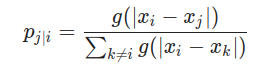
\includegraphics[width=100pt]{./img/reduction_dim/t_sne/eq_prob_1.png}
            \\
            Cela met à l'échelle toutes les valeurs pour que leur somme soit égale à 1. Il est important de remarquer que $p_{i|i}$ est évidement fixé à 0 et non à 1.

            
            \subsubsection*{Gérer des distances différentes}
            Si nous prenons deux points et essayons de calculer la probabilité conditionnelle entre eux, les valeurs de $p_{i|j}$ et $p_{j|i}$ seront possiblement différentes. En effet, elles proviennent de deux distributions différentes. Laquelle devons-nous donc choisir pour le calcul ?
            \\
            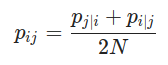
\includegraphics[width=100pt]{./img/reduction_dim/t_sne/eq_prob_2.png}
            \\
            Avec N le nombre de dimensions.
            \\
            \\
            Ainsi, nous avons tout mis à l'échelle de 1, la somme de tout est égale à 1. Mais nous avons ici simplifié la formule pour comprendre plus facilement comment cela focntionne, la formule originale dans le papier de recherche est la suivante : 
            \\
            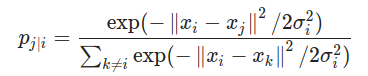
\includegraphics[width=100pt]{./img/reduction_dim/t_sne/eq_prob_3.png}
            \\







\subsubsection*{Perplexité}
En regardant cette formule, on remarque que :
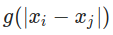
\includegraphics[width=100pt]{./img/reduction_dim/t_sne/eq_prob_4.png}
\\
équivaut à 
\\
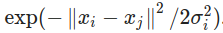
\includegraphics[width=100pt]{./img/reduction_dim/t_sne/eq_prob_5.png}
\\
Nous avons simplifié, car il serait difficile d'expliquer d'où vient $\sigma^2$ et quelle est la dépendance entre lui et nos clusters. On sait que la variance dépend de la gaussienne et du nombre de points entourant le centre de celle-ci. C'est ici qu'intervient la valeur de perplexité.
\\
La perplexité est plus ou moins un nombre cible de voisins pour notre point central. Fondamentalement, plus la perplexité est élevée, plus la variance a une valeur élevée. 
\\
Selon le papier original : "SNE effectue une recherche binaire de la valeur de sigma qui produit une distribution de probabilité avec une perplexité fixe qui est spécifiée par l'utilisateur".
\\
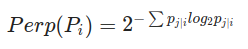
\includegraphics[width=100pt]{./img/reduction_dim/t_sne/eq_prob_6.png}
\\
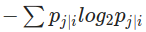
\includegraphics[width=100pt]{./img/reduction_dim/t_sne/eq_prob_7.png}
\\
C'est l'entropie de Shannon. La principale chose que l'on doit savoir est que la perplexité que l'on choisit est positivement corrélée avec la valeur de $\mu_i$ et pour la même perplexité, vous aurez plusieurs $\mu_i$ différents, basés sur les distances. La valeur de perplexité typique se situe entre 5 et 50.
\\
\\
\textbf{Intérpretation de la formule originale}
\\
\\
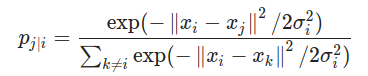
\includegraphics[width=100pt]{./img/reduction_dim/t_sne/eq_prob_8.png}
\\
Lorsque vous regardez cette formule, vous pouvez remarquer que notre gaussienne est convertie en : 
\\
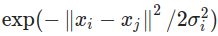
\includegraphics[width=100pt]{./img/reduction_dim/t_sne/eq_prob_9.png}
\\
Cela permet de distinguer les probabilités du voisin.





\subsubsection*{Créer un espace de faible dimension}
La partie suivante de t-SNE consiste à créer un espace de faible dimension avec le même nombre de points que dans l'espace original. Les points doivent être répartis de manière aléatoire dans le nouvel espace. 
\\
Le but de cet algorithme est de trouver une distribution de probabilité similaire dans l'espace à faible dimension. Le choix le plus évident pour la nouvelle distribution serait d'utiliser à nouveau les gaussiennes. Ce n'est malheureusement pas la meilleure idée. L'une des propriétés de la gaussienne est qu'elle a une "queue courte", ce qui crée un problème d'encombrement.
\\
Pour résoudre ce problème, nous allons utiliser la distribution t de Student avec un seul degré de liberté. Nous ne développerons pas notre choix ici par souci de simplicité, afin de se concentrer sur l'essentiel.
\\
Nous obtenons donc :
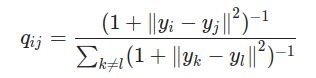
\includegraphics[width=100pt]{./img/reduction_dim/t_sne/eq_red_dim_1.png}
\\
Au lieu de :
\\
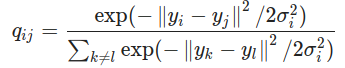
\includegraphics[width=100pt]{./img/reduction_dim/t_sne/eq_red_dim_2.png}
\\
Visuellment cela donne : 
\\
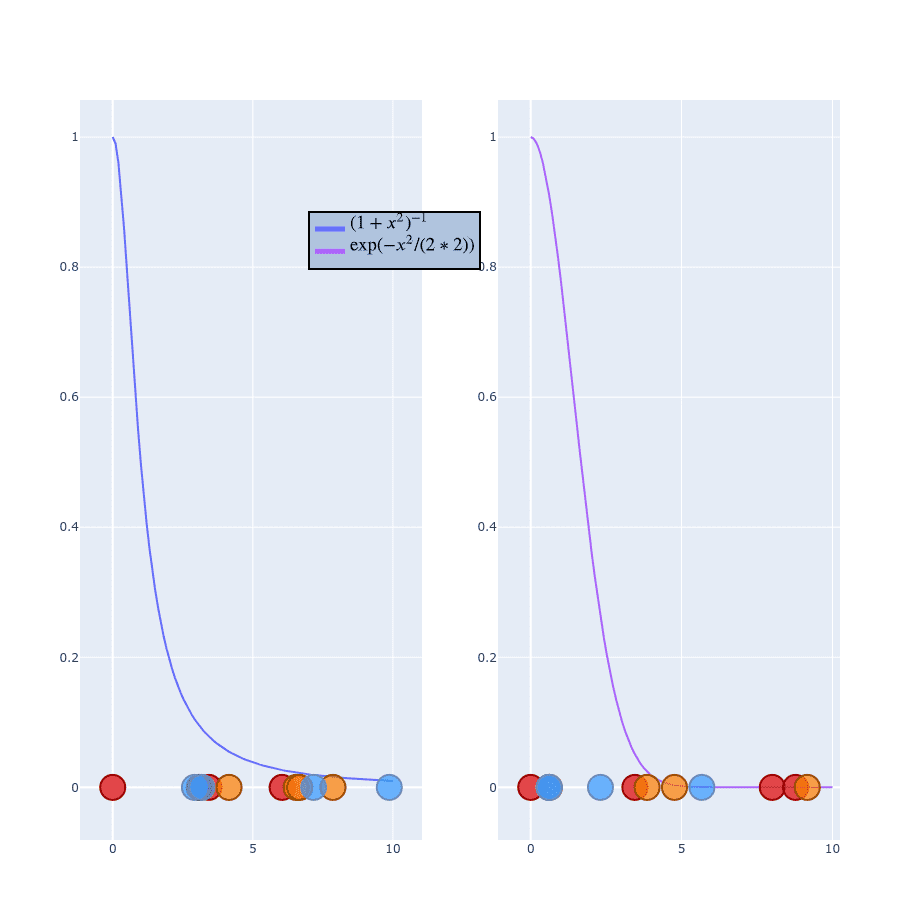
\includegraphics[width=\linewidth]{./img/reduction_dim/t_sne/graph.png}
\\
L'utilisation de la distribution de Student résout notre problème. Elle "tombe" rapidement et a une "longue queue", de sorte que les points ne seront pas écrasés en un seul point.
\\
Cette fois, nous n'avons pas à nous soucier de $\sigma^2$, car il n'y en a pas dans la formule de $q_{ij}$. Nous n'allons pas générer tout le processus de calcul de $q_{ij}$ car il fonctionne exactement de la même manière que $p_{ij}$. Voici les deux formules et passons à la suite :
\\
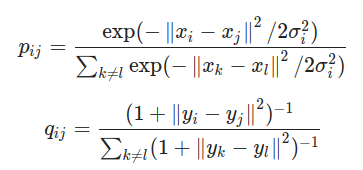
\includegraphics[width=\linewidth]{./img/reduction_dim/t_sne/eq_red_dim_3.png}
            





\subsubsection*{Déscente de gradient}
Pour optimiser cette distribution, t-SNE utilise la divergence de Kullback-Leibler entre les probabilités conditionnelles $p_{j|i}$ et $q_{j|i}$ :
\\
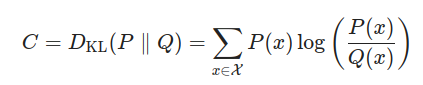
\includegraphics[width=\linewidth]{./img/reduction_dim/t_sne/desc_grad_1.png}
\\
Nous n'allons pas faire le calcul ici. Ce dont nous avons besoin, c'est de la dérivée :
\\
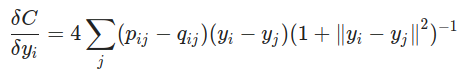
\includegraphics[width=\linewidth]{./img/reduction_dim/t_sne/desc_grad_2.png}
\\
Le gradient agit comme une répulsion et une attraction entre les points. Un gradient est calculé pour chaque point et décrit la "force" avec laquelle il doit être attiré et la direction qu'il doit choisir.
\\
\\
C'est une exagération t-SNE n'est pas aussi rapide. Nous avons sauté beaucoup d'étapes pour simplifier la compréhansion du processus.
\\
\\
Si l'on reprend les données de notre introduction, voici une résolution possible de t-SNE : 
\\
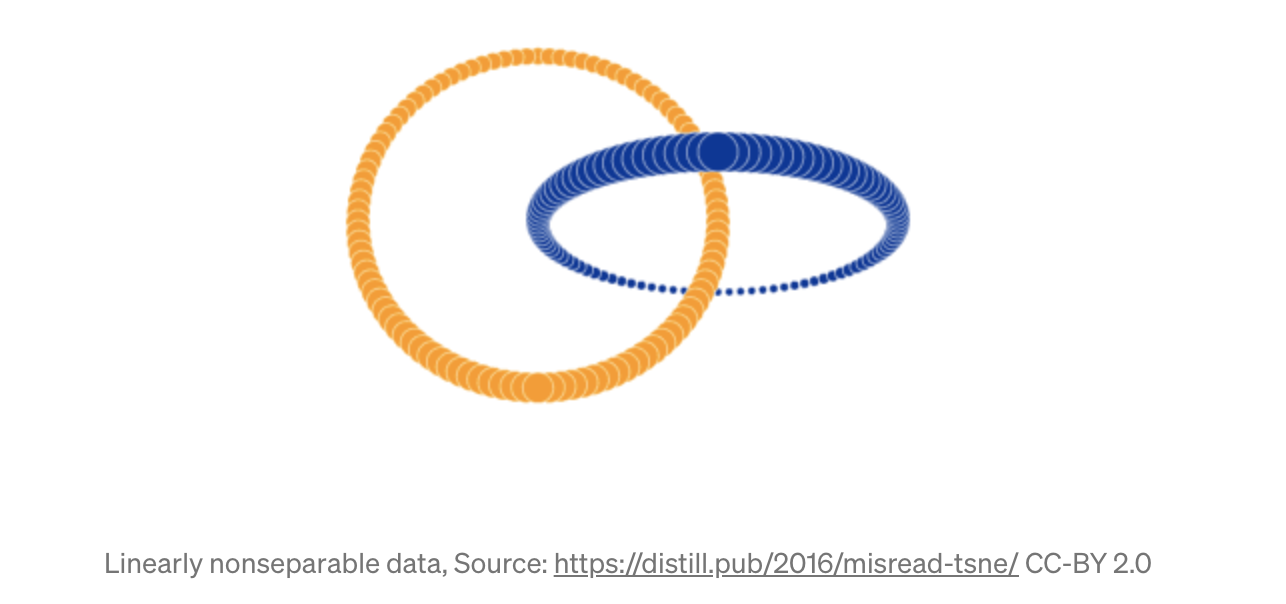
\includegraphics[width=\linewidth]{./img/reduction_dim/t_sne/exemple_data}
\\
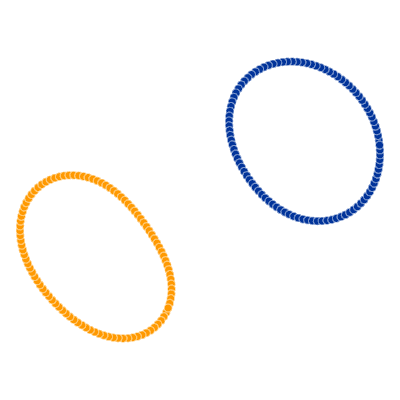
\includegraphics[width=\linewidth]{./img/reduction_dim/t_sne/exemple_data_2.png}
            


\subsubsection*{Conclusion}
Ici, nous avons vu que t-SNE distribue les clusters uniformément autour du centre, ce qui contribue à préserver la structure locale, mais au détriment d'informations sur la structure globale. 
\\
\\
t-SNE est un excellent outil pour comprendre et visualiser des ensembles de données à grande dimension, que celles-ci soient linéaires ou pas (contrairement à PCA).
\\
Néanmoin il au vu de son fonctionnement, il semble gourmant en ressource et implique de faible performance sur des jeux de données importants (à très grande dimension). C'est pourquoi il est souvent conseillé d'appliquer une PCA sur le jeu de données initial, afin de réduire celui-ci pour utiliser t-SNE.
\\
\\
Malgré les qualités évidentes de t-SNE, nous aimerions donc rechercher une autre méthode : plus performantes et surtout permettant de preserver au maximum la structure globale des données.
\\ 
C'est pourquoi nous nous interessons logiquement à UMAP.


        \newpage



        \subsection{Visualisation}
        En pratique (sur des exemples réels)
    


    \section{ => Motiver pour une autre possibilité}
    Pour la classification on peut parler des arbres de décisions qui de plus peuvent être interpréter et visualisé facilement.
    \\
    \\
    On aurait aussi pu parler d'autres algorithme comme LDA, SVD, ... 
